%Dokumentinnstillinger:---------------------------------
%Ved å google flitting kan du finne ut hva de forskjellige tingene her betyr, og hvordan du kan gjøre eventuelle endringer.
\documentclass[a4paper,11pt,norsk]{article}
\usepackage[utf8]{inputenc}
\usepackage{a4wide}
\usepackage{lmodern}
\usepackage[T1]{fontenc}
\usepackage{babel}
\setlength{\parindent}{0pt} 
\setlength{\parskip}{2ex}
\usepackage{fixltx2e}
\usepackage{amsmath}
\usepackage{amssymb}
\usepackage[pdftex, pdfborderstyle={/S/U/W 0}]{hyperref}
\usepackage{graphicx}
\usepackage[font=small,labelfont=bf]{caption}
\usepackage{tabularx}
\usepackage{multirow}
\usepackage[europeanresistors]{circuitikz}
\usepackage{tikz}
\usepackage{hyperref}
\usetikzlibrary{shapes,arrows}

\tikzset{
    opampdownlbl/.style={
        below,
        draw=none,
        append after command={
            (\tikzlastnode.north) edge ([shift={(-5pt, 0pt)}]\tikzlastnode.north)
                edge ([shift={(+5pt,0pt)}]\tikzlastnode.north)
        }},
    opampuplbl/.style={
        above,
        draw=none,
        append after command={
            (\tikzlastnode.south) edge ([shift={(-5pt,0pt)}]\tikzlastnode.south)
                edge ([shift={(+5pt,0pt)}]\tikzlastnode.south)
        }}
}
% Adds seperation between two elements with a comma. Format: "    ,    ".
\newcommand{\comma}{\quad , \quad}
% Gives double underline under selected text.
\def\dunderline#1{\underline{\underline{#1}}}
% Faster way to make an equation that can be formatted with "&" to look nice.
\def\spliteq#1{\begin{equation}\begin{split}{#1}\end{split}\end{equation}\\}
%------------------------------------- End -------------------------------------

\begin{document}

%Headingdel:---------------------------------------------
\begin{minipage}[c]{0.15\textwidth}

\includegraphics[width=2.0cm]{Design_projects/elsys_pos_staaende_ntnu.png} 
\end{minipage}
\begin{minipage}[c]{0.85\textwidth}

\renewcommand{\arraystretch}{1.7}
\large 
\begin{tabularx}{\textwidth}{|X|X|}
\hline
\multicolumn{2}{|l|}{} \\
\multicolumn{2}{|l|}{\huge \textbf{Designnotat}} \\
\multicolumn{2}{|l|}{}  \\
\hline
\multicolumn{2}{|l|}{Tittel: 
%Skriv inn tittel her:------------------------------------------
Trekantgenerator
} \\
\hline
\multicolumn{2}{|l|}{Forfatter: 
%Skriv inn forfattere her:--------------------------------------
Sindre Danielsen
} \\
\hline
%Skriv inn versjon og dato her her:-----------------------------
Versjon: 2.0 & Dato: 09.06.20
\\
\hline 
\end{tabularx}
\end{minipage}
\normalsize

%Automatisk generert innholdsfortegnelse:------------------

\setlength{\parskip}{0ex}
\renewcommand{\baselinestretch}{0.1}\normalsize
\tableofcontents
\renewcommand{\baselinestretch}{1.25}\normalsize
\setlength{\parskip}{2ex}
\rule{\textwidth}{1pt}

%Selve rapporten:------------------------------------------
\newpage
\section{Problembeskrivelse}
\label{sec:innledning}
Periodiske signaler fremkommer på flere former. Dette notatet gir en mulig løsning på hvordan et trekantsignal kan genereres. Trekantgeneratoren er vist i Figur~\ref{fig:triangularGenerator}.  \\
\begin{figure}[htbp]
    \centering
    \begin{circuitikz} [american voltages, european resistors, baseline=(current bounding box.center)]
        \ctikzset { label/align = straight }
        \draw
        % Bottom-right side
        % V trekantsignal
        (4, 2) to[short, -o] (5,2)
        to[short] (6,2)
        % V_
        (2,0) to[short] (2,-1)
        to[short,l=$V_-$,-o] (2,-1)
        % V+
        (2,4) to[short] (2,5)
        to[short, l=$V_+$,-o] (2,5)
        ;
        \node at (5,2.5) (PSU_l){$V_{\triangle}(t)$};
        
        
        % Nivåregulator
        \node[draw,minimum width=4cm,minimum height=4cm,anchor=south west] at (0,0){\textbf{Trekantgenerator}};

        
    \end{circuitikz}
    \caption{Trekantgenerator: Omformer to omvendte statiske signal til et trekantsignal.}
  \label{fig:triangularGenerator}
\end{figure} \\
Her vises to inngangsignaler $V_-$ og $V_+$ som er like statiske signaler, men motsatt retning. Trekantgeneratoren sender ut et trekantsignal $V_\triangle (t)$ basert på $V_-$ og $V_+$.
\\\\
Kravet for systemet er å ikke overskride et maksimalt frekvensavvik på  $\Delta f_{max} = 10\:000$\:ppm. \\
Frekvensendringen $\Delta f = f_0 - f$ må oppfylle:
\\
\begin{equation}
    \frac{|\Delta f|}{f_0} \leq \frac{\Delta f_{max}}{10^6} \textit{ , }
    \label{eq:max_freq}
\end{equation}
\\
der $f_0$ er den valgte frekvensen for systemet og $f$ er den målte frekvensen. \\\\

\textbf{Merk at}\label{note:amplitude_less} amplituden til trekantsignalet vil bli mindre enn amplituden til inngangsignalene, siden signalet svekkes når det beveger seg gjennom kabler og over motstander.
\newpage
\section{Prinsipiell løsning}
\label{sec:prinsipielllosning}

Trekantgeneratoren utvikles ved hjelp av to apparater vist i figur~\ref{fig:kretsElementer}.
\begin{figure}[htbp]
    \centering
    \begin{circuitikz} [american voltages, european resistors, baseline=(current bounding box.center)]
        \ctikzset { label/align = straight }
        \draw
        %Komperator
        % V_
        (6.4,-0.90) to[short] (6.4,-1.90)
        to[short,l=$V_-$,-o] (6.4,-1.90)
        % V+
        (6.4,2.9) to[short] (6.4,3.9)
        to[short, l=$V_+$,-o] (6.4,3.9)
        % Between systems
        (9.25, 1.8) to [open,v=$\mathbf{V_{\square} (t)}$] (9.25,0.2)
        %Top between systems
        (8.5,2) to[short,-o] (9.25,2)
        (9.25,2) to[short] (10,2)
        
        %Bottom between systems
        (8.5,0) to[short,-o] (9.25,0)
        (9.25,0) to[short] (10,0)
        % Integrator
        % V_
        (12,-0.90) to[short] (12,-1.90)
        to[short,l=$V_-$,-o] (12,-1.90)
        % V+
        (12,2.9) to[short] (12,3.9)
        to[short, l=$V_+$,-o] (12,3.9)
        % Top-right side
        (15.5,2) to[short, -o] (14.75,2)
        to[short] (14, 2)
        (14.75, 1.8) to [open,v=$\mathbf{V_\triangle(t)}$] (14.75,0.2)
        % Bottom-right side
        (15.5, 0) to[short, -o] (14.75,0)
        to[short] (14,0);
        
        % Nivåregulator
        \node[draw,minimum width=4cm,minimum height=3.8cm,anchor=south west] at (4.5,-0.90){\textbf{Komparator}};
        \node[draw,minimum width=4cm,minimum height=3.8cm,anchor=south west] at (10,-0.90){\textbf{Integrator}};

        
    \end{circuitikz}
    \caption{Komparator: Firkantsignal $\mathbf{V_{\square} (t)}$, Integrator: Integrerer $\mathbf{V_{\square} (t)}$ til trekantsignal $\mathbf{V_\triangle(t)}$.}
  \label{fig:kretsElementer}
\end{figure} \\
Fra figuren ser vi at både komparatoren og integratoren tar samme inngangssignaler $V_-$ og $V_+$ som trekantgeneratoren. \\
\newpage
En foreslått kretstopologi til et slikt system er vist ved Figur~\ref{fig:kretsTopologi}. \\
\begin{figure}[htbp]
    \centering
    \begin{circuitikz}
        % Circuit to comparator
        \draw(0, 0)
        to[short,-o] (1,0)
        node[below]{$v_3$}
        to[short] (1.5,0)
        (2.70,-0.490) node[op amp ,yscale =-1] (opamp) {}
        (opamp.up) ++ (0,-.5) node[opampdownlbl]  {$V_-$} -- (opamp.up)
        (opamp.down) ++ (0,.5) node[opampuplbl]  {$V_+$} -- (opamp.down)
        ;
        % Grounding op-amp
        \draw (1.505,-0.97) to (1.505,-1.25) node[ground]{}; 
        ;
        % All except op-amp
        \draw (1,0)
        % R2
        to[short,o-] (1,2)
        to[R=$R_2$] (3.90,2)
        to[short,-o] (3.90,-.5)
        node[below]{$v_1$}
        % Between comparator and integrator
        to[short] (6.9,-.5)
        % R
        to[R=$R$,-o] (8.9,-.5)
        
        % Integrator
        (10.15,-0.989) node[op amp ,yscale =1] (opamp) {}
        ;
        % Grounding Integrator
        \draw (8.95,-0.97-0.5) to (8.95,-1.25-0.5) node[ground]{}; 
        ;
        % C
        \draw (8.90,-0.5)
        to[short,o-] (8.90, 1.5)
        to[C=$C$] (11.4,1.5)
        to[short,-o] (11.4, -1)
        to[short] (11.4, -3.5)
        to[short] (0, -3.5)
        to[R=$R_1$] (0,0)
        ;
        \draw (12.9, -1) to[short,-o] (11.4,-1);
        \draw(12.9,-1) to[short,-o] (12.9,-1)
        node[below]{$v_2$};
        
        \node[draw,dashed,minimum width=5.25cm,minimum height=8.0cm,anchor=south west, label={Komparator}] at (-1,-5) ;
        \node[draw,dashed,minimum width=5.25cm,minimum height=8.0cm,anchor=south west, label={Integrator}] at (6.5,-5);

        \end{circuitikz}
    \caption{Forslag til kretstopologi for trekantgenerator.}
    \label{fig:kretsTopologi}
\end{figure}
\\

I teorien kansellerer $V_-$ og $V_+$ hverandre, som gir $v_1 = 0$V, mens i praksis, så forekommer det ulikheter mellom $V_+$ og $V_-$, slik at det blir et utgangssignal på op-ampen $V_\square (t) = v_1$ \\(Forklart grundigere av referansevedleggene \cite{komparator} og \cite{komparator_vid}):
\\
\begin{equation}
 v_1 = 
\left\{\begin{matrix}
    \textit{ \: } V \quad \textit{for \:} v_3 > 0 \\
    -V \quad \textit{for \:} v_3 < 0
\end{matrix}\right .
\label{eq:square}
\end{equation}
\\
Den tiden det tar før op-ampen virker slik, er avhengig av op-ampens egenskaper, som man finner under \emph{stigrate} $SR$ i datablad til komponenten. Stigetiden for dette tilfellet er:
\\
\begin{equation}
    T_s = \frac{2V}{SR}
    \label{eq:T_s}
\end{equation}
\\
Dersom $|v_1| > 0$V, så vil op-ampen begynne å regulere forskjellen på dens $+$ og $-$ pol, slik at signalet vil skifte mellom negativ og positiv $V$. 
\newpage
Komparatoren er koblet med en feedback på utgangen $v_1$, som betyr at det vil gå et \\ signal gjennom motstanden $R_2$. Inngangssignalet $v_3$ er gitt av spenningsdelingen: \\
\begin{equation}
    v_3 = \frac{R_1}{R_1+R_2}(v_1 - v_2)
    \label{eq:spenningsdeling}
\end{equation}
\\\\
Integratoren trekker på signalet $v_1$ gjennom motstanden $R$, slik at kondensatoren $C$ vil utvikle et trekantsignal $V_\triangle (t) = v_2$:
\\
\begin{equation}
    v_2(t) = v_2 (0) - \frac{1}{\tau} \int^t _0 v_1 (t) dt
    \quad , \quad \tau = RC\textit{.}
\label{eq:integral}
\end{equation}
\\
\textbf{Merk at } det er underforstått at spenningsforsyningene $V_-$ og $V_+$ til op-ampen gjelder både op-ampen i komparatoren og integratoren.
\\\\
For å forklare at et firkantsignal integreres til et trekantsignal, så er det tre tilfeller å ta for seg. \\
Når $v_1 > 0$V, så vil signalet integreres bli en stigende linje. \\
Når $v_1 < 0$V, gir en synkende linje. \\
Når $v_1 = 0$V, gir topp-/bunnpunktet, gitt at $|v_1| > 0$V for tiden før. \\
Dette kan bli observert på oscilloskop-bildet i figur~\ref{fig:bb_trekantsignal}.
\newpage
\begin{figure}[htbp]
    \centering
    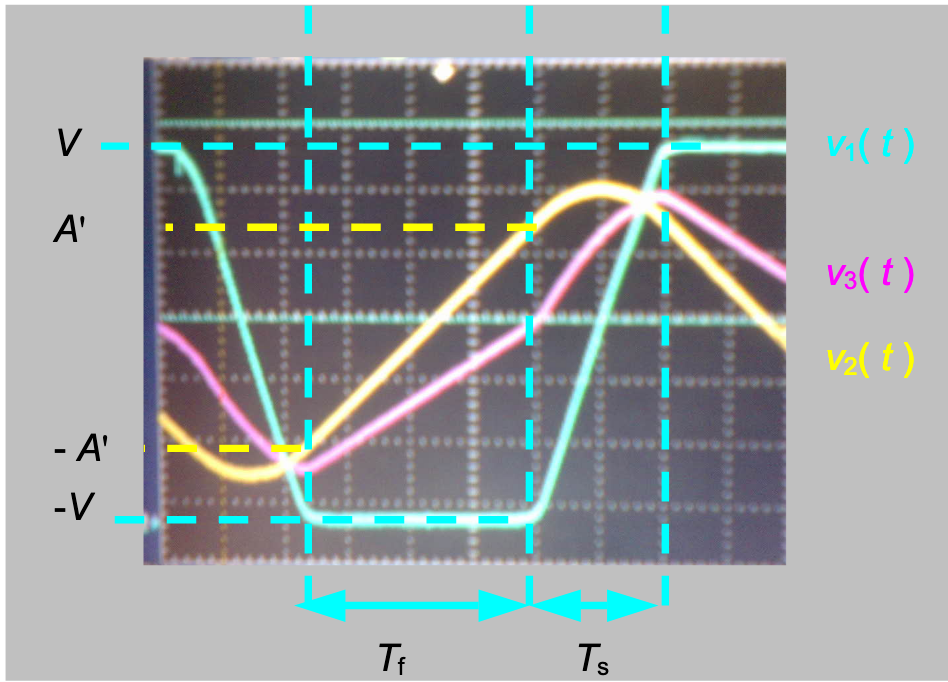
\includegraphics[width=1.0\textwidth]{img/avbildning.png}
    \caption{Signalene for komparatoren og integratoren \cite{bb_trekantsignal}.}
    \label{fig:bb_trekantsignal}
\end{figure}
\\
Symbolene og deres funksjonalitet fra figuren forklares i vedlegg~\ref{at:A}.


\newpage

\section{Realisering og test}
\label{sec:realisering}
Når systemet utvikles, så avhenger motstandsverdiene fra kretsen i  figur~\ref{fig:kretsTopologi} av frekvensen $f_0$ på signalet.
Verdiene brukt i systemet er fremvist i tabell~\ref{table:variabler}.
\\
\begin{table}[htbp]
\centering
\begin{tabular}{ |c|c|c|c| } 
\hline
\textbf{Navn} & \textbf{Verdi} & \textbf{Beskrivelse}\\
\hline
$f_0$ & $3.50000$kHz & Teoretisk ønsket frekvens  \\
\hline
$f$ & $3.49145$kHz & Målt frekvens \\
\hline
$R$ & $1000 \Omega$ & Teoretisk valgt motstand.  \\ 
\hline
$R_1$ & $1000 \Omega$ & $R_1 = R \implies $ ingen forsterkning. \\ 
\hline
$R_2$ & $1410\Omega$ & Målt med potensiometer \\
\hline
$C$ & $1\mu$F & Teoretisk kondensator \\
\hline
$V_+$ & $5$V & Op-amp spenningskilde \\
\hline
$V_-$ & $-5$V & $V_- = -V_+$ \\
\hline
Op-amp & LF353P & \\

\hline
\end{tabular}
\caption{Verdiene brukt i realisering av systemet.}
\label{table:variabler}
\end{table}
\\
\begin{figure}[htbp]
    \centering
    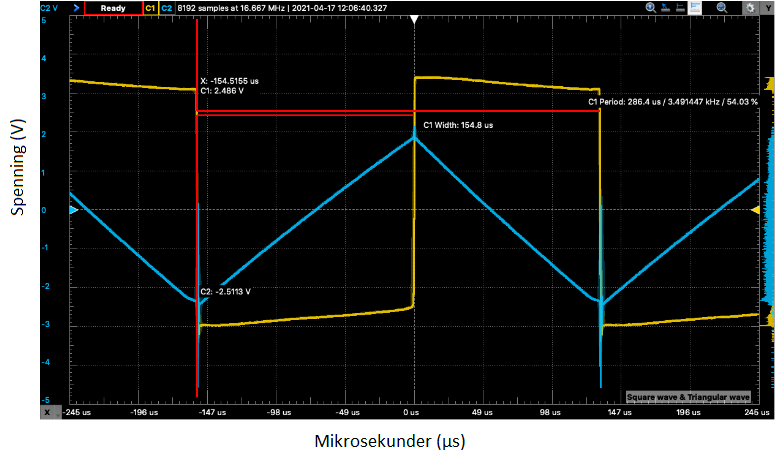
\includegraphics[width=1.0\textwidth]{img/Oscilloskop.png}
    \caption{Blå funksjon: $V_\triangle (t)$, Gul funksjon: $V_\square (t)$}
    \label{fig:triangularWave}
\end{figure}
\\
\newpage
Verdiene til motstandene er de teoretiske verdiene, som vi har valgt til å være 1k$\Omega$, og bruker et potensiometer på $R_2$ for å få en mest nøyaktig mulig $f_0$. Det er fordi kabler har motstand, samt motstandene har avvik på: $R_{1_a} = 7\Omega$, $R_{a} = 10\Omega$ og $R_{2_a} = 10\Omega$ samt at kondensatoren ikke er ideell. Siden frekvensen er bestemt fra RC-kretsen i figur~\ref{fig:kretsTopologi}. Vi har valgt å finne motstandsverdiene eksperimentelt.
Figur~\ref{fig:triangularWave} viser en avbildning av firkantsignalet og trekantsignalet som den reelle kretsen i figur~\ref{fig:realKrets} gir. Den målte frekvensen $f$ fra figuren er skrevet opp i tabell~\ref{table:variabler}.
\\\\
Bruker likning~\ref{eq:max_freq} for å sjekke om systemet er innenfor kravet:
\\
\begin{equation}
    \frac{|\Delta f|}{f_0} = 0.00244 < 0.01 \textit{.}
    \label{eq:systemkrav_godkjent}
\end{equation}
\\
Denne realiseringen av systemet er innenfor systemkravet som er satt i seksjon~\ref{sec:innledning}.
\\\\
Oscilloskop-bildet viser ''humper'' på topp-/bunnpunktene til trekantsignalet. \\
Kort sagt, så kommer dette av at signalet som blir utviklet er en parabel. Der størrelsen på ''humpene'' er gitt av likning~\ref{eq:amplitude_hump}. 
Forklaring og fremgangsmåten kommer frem i Vedlegg~\ref{at:A}.
\\\\
Høyden på amplitude-tillegget $\Delta A$ er neglisjerbar for lave frekvenser og raske op-amper, som også kan observeres ved likning~\ref{eq:amplitude_hump}. \\
Dette fordi $\Delta A$ er omvendt proporsjonal med $\tau$ og $SR$, der $\tau$ bestemmes av frekvensen på signalet over kondensatoren $C$ når det er vekselspenning.

\\\\
Slik nevnt i seksjon~\ref{note:amplitude_less}, 
så får vi $V_\triangle(t) < V_\square(t)$ som vist ved figur~\ref{fig:triangularWave}.
\newpage
Den oppkoblede kretsen som gir oscilloskop-avbildningen i figur~\ref{fig:triangularWave} er vist i figur~\ref{fig:realKrets}.

\begin{figure}[htbp]
    \centering
    \includegraphics[width=1.0\textwidth]{img/RealKrets.jpg}
    \caption{Reell krets av systemet.}
    \label{fig:realKrets}
\end{figure}
\\
I figuren blir det brukt et potensiometer for $R_2$ som går fra 8$\Omega$ til 10k$\Omega$, fordi det er lettere å finne en ønsket motstandsverdi.
\newpage

\section{Konklusjon}
\label{sec:konklusjon}
I dette notatet er det utviklet et trekantsignal fra to statiske inngangsignaler $V_-$ og $V_+$.
Dette er gjort ved help av en komparator og en integrator.
\\\\
Vi har funnet at trekantsignalet styrke er redusert fra firkantsignalet. Trekantsignalet har også forstyrrelser ved dens topp-/bunnpunkt.
\\\\
En eventuell forbedring av systemet er bruk av en buffer mellom komparatoren og \\ integratoren for å få en lik amplitude på trekantsignalet som firkantsignalet.
For å bli kvitt eller redusere effekten av $\Delta A$, så kan en raskere op-amp brukes, og/eller lavere frekvenser på signalet.
\\\\
Fra likning~\ref{eq:systemkrav_godkjent} ser vi at systemet lever opp til systemkravet fra seksjon~\ref{sec:innledning}.

\section{Takk}
Takk til Håvard Romsaas og Jo Vegard Molvik for godt samarbeid under prosjektet.
\newpage

%Bibliografi: Legg til flere elementer ved å legge til flere \bibitem:--------
\phantomsection
\addcontentsline{toc}{section}{Referanser}
\begin{thebibliography}{99}

\bibitem{komparator}
    \emph{'Komparator - Comparator'} (2021). Wikipedia\\
    Tilgjengelig ved: \href{https://no.qaz.wiki/wiki/Comparator}{https://no.qaz.wiki/wiki/Comparator}
    \\ (Sist åpnet: 25. April 2021).

\bibitem{komparator_vid}
    EzEd Channel (2019), Video \\
    \emph{Op-Amp as a WAVEFORM GENERATOR - Applications of OpAmp - BEE} \\
    Tilgjengelig ved: \href{https://www.youtube.com/watch?v=HJKFXmJVwaA}{https://www.youtube.com/watch?v=HJKFXmJVwaA} \\
    (Sist åpnet: 25. april 2021)

\bibitem{bb_trekantsignal}
    Teknisk notat: 'Trekantgenerator', \\
    Figur 2: \emph{'Interne signal i trekantgeneratoren.'} (Torstein Bolstad, NTNU 2020, s.3). \\
    (Sist åpnet: 25. april 2021)




\end{thebibliography}

\appendix
%Tillegg. Flere tillegg legges til ved å lage flere sections:-----------------
\newpage
\section{Årsaken til et uperfekt trekantsignal}\label{at:A}
Ser på tilfellet der $v_1(t) = V_+$, slik at integratoren vil generere en rett linje, så gir likning~\ref{eq:integral}:
\\
\begin{equation}
    v_2(t) = v_2(0) - \frac{V}{\tau}t \textit{.}
    \label{eq:integral_V}
\end{equation}
\\
Siden op-ampene har en symmetrisk forsyningspenning $V_+$ og $V_-$, så kan vi anta at det genererte signalet vil være symmetrisk om tidsaksen. Slik at $v_2(T_f) = v_2(0)$.
Ved innsetting i likning~\ref{eq:integral_V}, så har vi at
\\
\begin{equation}
    T_f = \frac{2v_2(0)}{V}\tau \textit{,}
    \label{eq:T_f}
\end{equation}
\\
der $T_f$ representerer tidsintervallet i figur~\ref{fig:bb_trekantsignal} når firkantsignalet er på sin min.-/maks. verdi \\ (respektivt $V_-$/$V_+$).
\\\\
Vi kan finne $v_2(0)$ ved å bruke likning~\ref{eq:spenningsdeling} sammen med likning~\ref{eq:integral} og likning~\ref{eq:T_f}, der $v_1(T_f) = V_+$ og $v_3(T_f) = 0$, slik at
\\
\begin{equation}
    v_2(0) = \frac{R_1}{R_2}V \textit{.}
    \label{eq:v_0}
\end{equation}
\\
Kan da utvikle likning~\ref{eq:T_f} til
\\
\begin{equation}
    T_f = 2 \frac{R_1}{R_2}\tau \textit{.}
\end{equation}
\\
Analytisk så er det en fordel å sette $t = 0$ ved starten av intervallet $T_s$ fra figur~\ref{fig:bb_trekantsignal} slik at $v_1(t)$ blir
\\
\begin{equation}
    v_1(t) = V_- + \frac{2V}{T_s}t \quad , \quad t\in<T_f, T_s]\\
\end{equation}
\\
\newpage
Likning~\ref{eq:integral} gir da at
\begin{equation}
    v_2(t) = v_2(0) + \frac{V}{\tau}\left ( t - \frac{t^2}{T_s} \right ) \textit{,}
\end{equation}
\\
som er en parabel med toppunkt midt i tidsintervallet, slik at
\\
\begin{equation}
    v_2\left( \frac{T_s}{2} \right) = v_2(0) + \frac{VT_s}{4\tau} \textit{.}
\end{equation}
\\
For å få flere kjente verdier, så kan vi utvikle den videre ved hjelp av likning~\ref{eq:T_s}:
\begin{equation}
    v_2\left( \frac{T_s}{2} \right) = v_2(0) + \frac{V^2}{2\tau SR} \textit{.}
\end{equation}
\\
Det vi ser er at parabelen sørger for at trekantsignalet ikke er perfekt ved topp-/bunnpunktet, som  her utvikler en ''hump''. Størrelsen på den er gitt ved likning~\ref{eq:amplitude_hump}.
\\
\begin{equation}
    \Delta A = \frac{V^2}{2\tau SR} \textit{.}
    \label{eq:amplitude_hump}
\end{equation}
\\
Den totale høyden på signalet her er da gitt av
\\
\begin{equation}
    A = v_2(0) + \Delta A \textit{.}
    \label{eq:amplitude_total}
\end{equation}
\\
Denne uønskede hendelsen observeres også i realiseringen av kretsen vist ved  figur~\ref{fig:triangularWave}.
\section{Vurdering}
Teksten ser ut til å være forklarende, samt så presis som mulig.
Figurene er beskrivende for hva som foregår i teksten.
Variabler i figurer og likninger blir forklart.
Figurer, likninger og tabeller er nummerert og har referanser der det passer og er beskrivende.
Påstander ser ut til å bli forklart.
Kun det essensielle matematisk kommer frem i prinsipiell løsning, fremgangsmåter er lagt til vedlegg dersom man ønsker nøyere lesning.
Konklusjonen er kort oppsummerende og forklarer det vi er kommer frem til og mulige forbedringer.
\section{Tilbakemelding}
\begin{itemize}
    \item Er teksten forklarende nok, eller er det noe som kunne utdypes mer?
    \item Er det lurt å legge den lange matematiske forklaringa til i et vedlegg, slik jeg gjorde (uperfekt trekantsignal) ?
    \item Er det prossessfokus, eller var det skrevet slik vi burde?
    \item Burde jeg ha tegnet opp hva som er hva på den reelle kretsen, eller går det greit å la være?
    \item Er referansene greit brukt?
\end{itemize}



\end{document}